\documentclass[tikz,border=10pt]{standalone}
\usetikzlibrary{angles}
\begin{document}
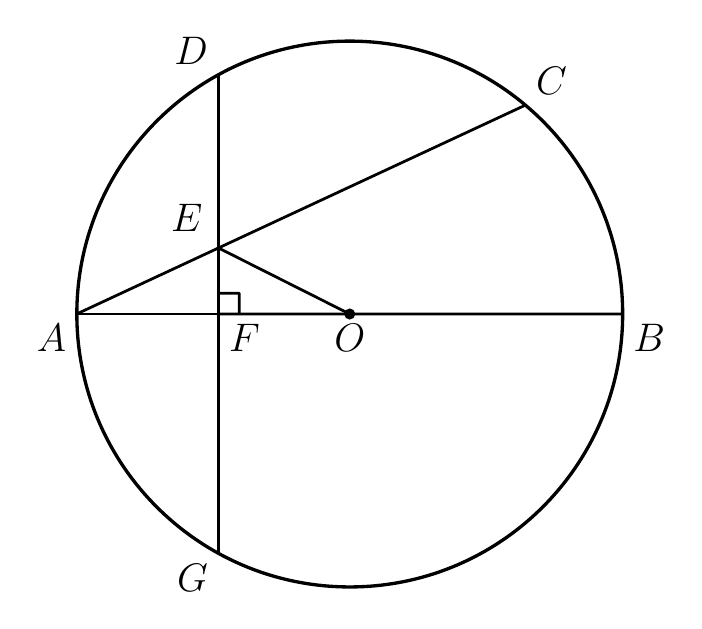
\begin{tikzpicture}[line join=round, line width=1.0pt,
  lbl/.style={font=\fontsize{14.5}{17.4}\selectfont}]
\coordinate (A) at (-3.492,0.009);
\coordinate (B) at (3.441,0.009);
\coordinate (C) at (2.206,2.661);
\coordinate (D) at (-1.692,3.047);
\coordinate (F) at (-1.692,0.009);
\coordinate (G) at (-1.692,-3.032);
\coordinate (O) at (-0.025,0.008);


\coordinate (E) at (-1.692,0.847);


\draw[line width=1.2pt] (O) circle[radius=3.466];


\draw (A) -- (F) -- (B);
\draw (O) -- (B);
\draw (F) -- (O);


\draw (D) -- (E) -- (F) -- (G);
\draw (D) -- (F) -- (G);


\draw (A) -- (E) -- (C);
\draw (E) -- (O);


\draw pic[draw, angle radius=0.264cm] {right angle=D--F--O};


\fill (O) circle (2.000pt);


\node[lbl, below left]  at (A) {$A$};
\node[lbl, below right] at (B) {$B$};
\node[lbl, above right] at (C) {$C$};

\node[lbl, above left] at (D) {$D$};
\node[lbl, anchor=south east, xshift=-2pt, yshift=2pt] at (E) {$E$};
\node[lbl, below right] at (F) {$F$};

\node[lbl, below left] at (G) {$G$};
\node[lbl, below]       at (O) {$O$};
\end{tikzpicture}
\end{document}